\documentclass{ctexart}
\usepackage{amsmath}
\usepackage{graphicx}
\def\dd{{\rm d}}
\begin{document}
\title{计算物理作业 3}
\author{刘畅, PB09203226}
\maketitle

{\bf[作业3]}:\quad 在球坐标系 $(\rho,\theta,\phi)$
下产生球面上均匀分布的随机坐标点,给出其直接抽样方法。

\section{算法}
球面上的均匀分布满足
\[
\frac{1}{4\pi}\dd \Omega = \frac{1}{4\pi}\sin\theta\dd\theta\dd\phi
\]
因此概率密度函数
\[
p(\theta,\phi) = \frac{1}{4\pi}\sin\theta = \frac{\sin\theta}{2}\cdot
\frac{1}{2\pi} = p(\theta)\cdot p(\phi)
\]
因此 $\theta$ 和 $\phi$ 是独立的两个随机变量. 积累函数
\[
\xi(\theta) = \int^\theta_0 \frac{\sin\theta}{2}\dd\theta
= \frac{1-\cos\theta}{2}
\]
\[
\xi(\phi) = \frac{\phi}{2\pi}
\]
因此对于 $[0,1]$ 上满足均匀分布的点列 $\xi$, 变换
\[
\theta(\xi) = \arccos(1-2\xi)
\]
\[
\phi(\xi) = 2\pi\xi
\]
就得到单位球面上的均匀分布.

\section{程序}
程序非常直接, 按照前面的算法编码, 首先需要 $[0,1]$ 上的均匀分布:
\begin{verbatim}
/* uniform distribution over [0,1] */
double rand_norm(void)
{
    return (double) rand() / (double) RAND_MAX;
}
\end{verbatim}
然后需要前面的变换函数:
\begin{verbatim}
double theta(double xi)
{
    return acos(1 - 2*xi);
}

double phi(double xi)
{
    return 2 * CONST_PI * xi;
}
\end{verbatim}
最后生成球面上的均匀分布数据点:
\begin{verbatim}
int main(void)
{
    srand(time(NULL));    /* init rand nr. gen. */
    for (i = 0; i < NSTEPS; i++) { /* generate dataset */
        t = theta(rand_norm());
        p = phi(rand_norm());
        printf("%.12f %.12f %.12f\n",
               sin(t)*cos(p), sin(t)*sin(p), cos(t));
    }
}
\end{verbatim}

\section{结果}
运行这个程序, 将结果作图. 如下:
\begin{center}
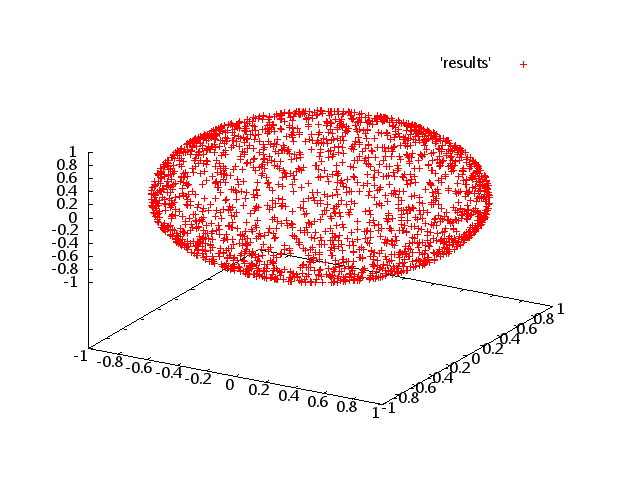
\includegraphics[width=4.6in]{sphere.png}
\end{center}
由于这是三维空间到二维平面的投影, 因此球面看起来像一个椭球面.
可以直观地看出这是一个均匀分布.

\end{document}